\documentclass[../Main.tex]{subfiles}
\begin{document}

    \section{Generación de texto}
    
    \begin{justify}
    En esta sección se describe brevemente el funcionamiento del modelo generador GPT-2 que fue el seleccionado en el proyecto para la tarea de generar texto.
    
    La forma más sencilla de ejecutar un modelo GPT-2 entrenado es permitir que divague por sí solo (lo que técnicamente se llama Generating Unconditional Samples); alternativamente, se le puede dar un mensaje para que genere sobre un tema determinado (también conocido como Generating Interactive Conditional Samples). En el caso de divagaciones, simplemente se entrega el token de inicio y se hace que comience a generar palabras (el modelo entrenado usa <|endoftext|> como su token de inicio. En las siguientes figuras se mostrará como <s>) \cite{46}. %https://jalammar.github.io/illustrated-gpt2/
    
    En el caso del proyecto al modelo GPT-2 se le pasó un mensaje inicial (oración) para que generara a partir de ese mensaje el texto (Generating Interactive Conditional Samples).
    \end{justify}
    
    \begin{figure}[H]
	\begin{Center}
		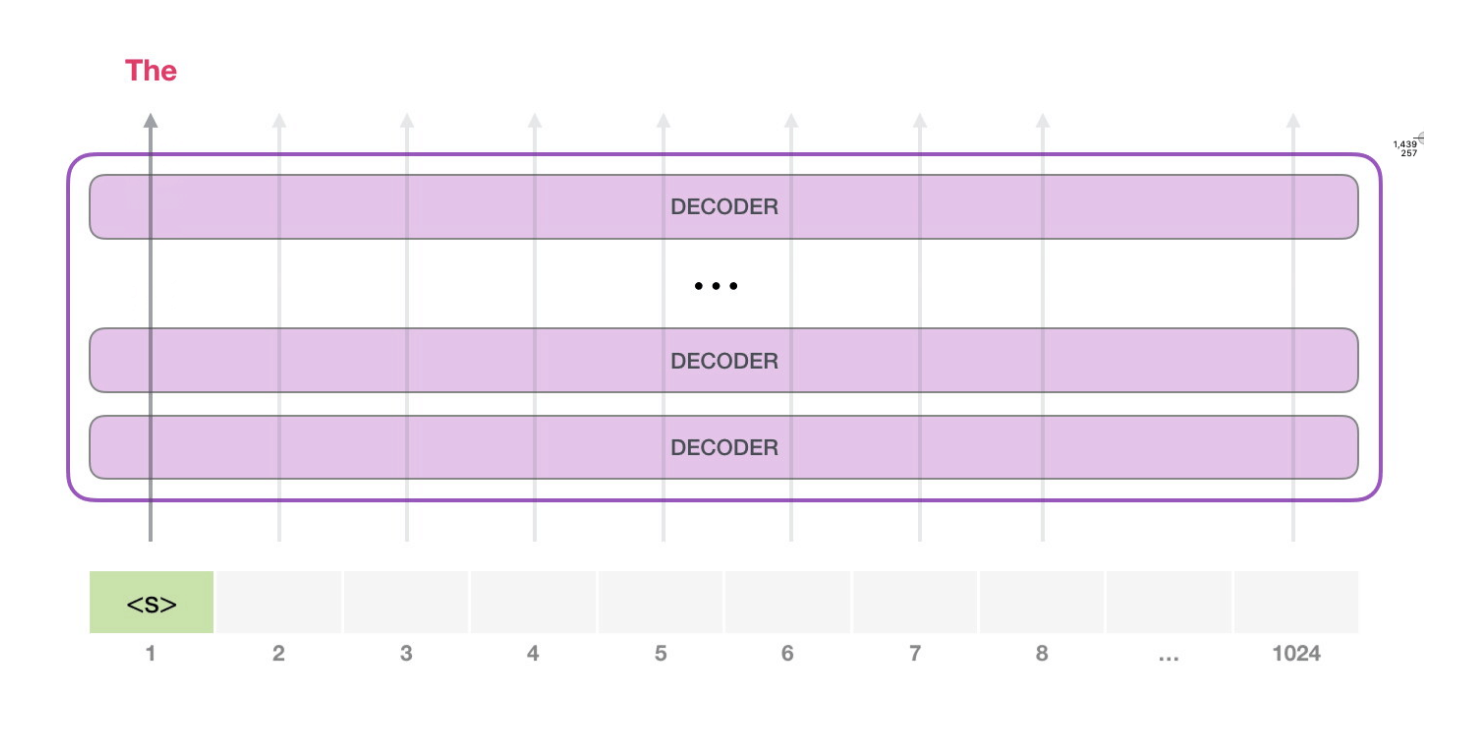
\includegraphics[width=6in,height=3in]{Chapters/04ChapterModelamiento/images/gpt-2-layers-input-1.png}
	    \caption{Ejemplo entrada activa GPT-2}
	    Fuente: The Illustrated GPT-2 \cite{46}
        \label{fig:section}
	\end{Center}
    \end{figure}
    
     % Revisar los siguientes enlaces para la información de esta sección
     % https://blog.floydhub.com/gpt2/
     % https://openai.com/blog/better-language-models/
     % https://openai.com/blog/gpt-2-1-5b-release/
     
    
    \begin{justify}
     El modelo solo tiene un token de entrada, por lo que esa ruta sería la única activa. El token se procesa sucesivamente a través de todas las capas, luego se produce un vector a lo largo de ese camino. Ese vector se puede puntuar con el vocabulario del modelo (todas las palabras que conoce el modelo, 50.000 palabras en el caso de GPT-2). En este caso se selecciona el token con mayor probabilidad. GPT-2 tiene un parámetro llamado top-k utilizado para que el modelo considere el muestreo de palabras distintas de la palabra superior (cuando top-k = 1) \cite{46}.
     
     En el siguiente paso, se agrega la salida del primer paso a la secuencia de entrada para que el modelo haga su próxima predicción:
    \end{justify}
    
    \begin{figure}[H]
	\begin{Center}
		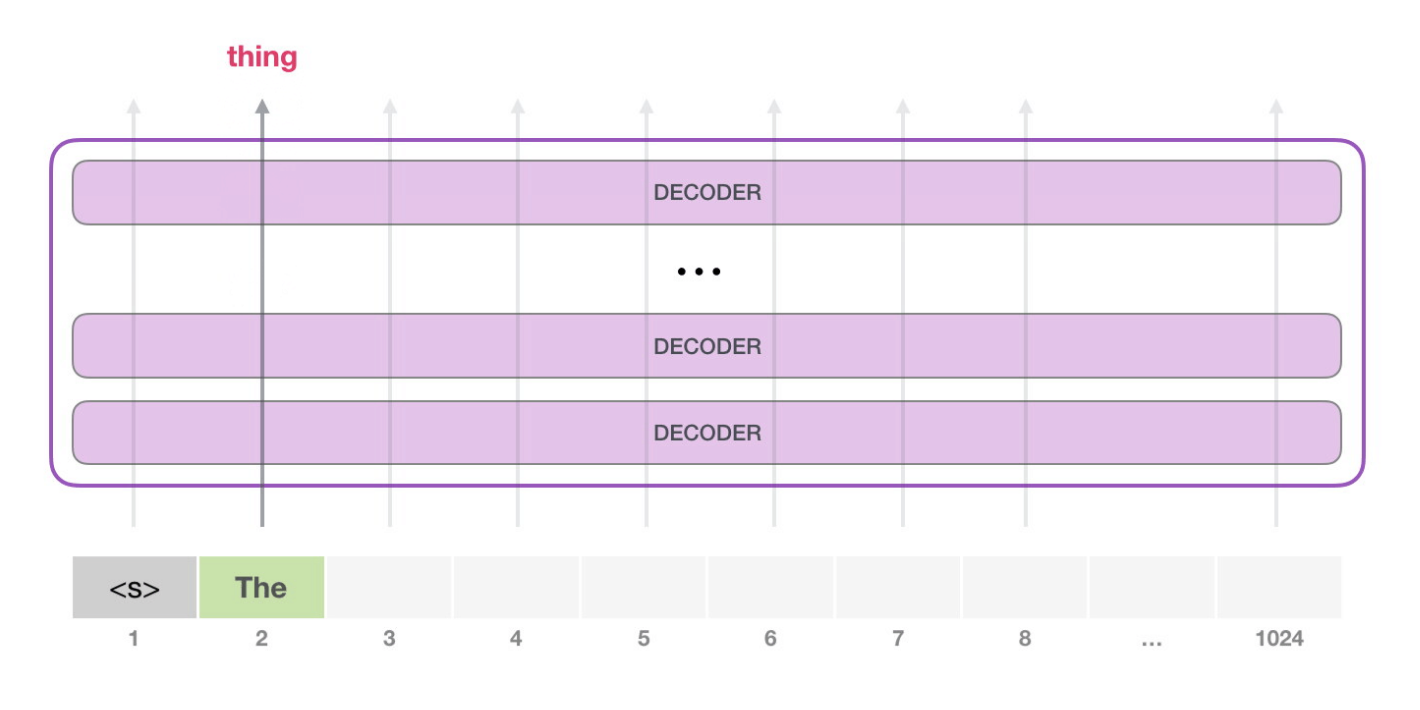
\includegraphics[width=6in,height=3in]{Chapters/04ChapterModelamiento/images/gpt-2-layers-input-2.png}
	    \caption{Ejemplo 2 entrada activa GPT-2}
	    Fuente: The Illustrated GPT-2 \cite{46}
        \label{fig:section}
	\end{Center}
    \end{figure}
    
    \begin{justify}
    La segunda ruta es la única que está activa en este cálculo. Cada capa de GPT-2 ha conservado su propia interpretación del primer token y lo usará para procesar el segundo token. GPT-2 no reinterpreta el primer token a la luz del segundo token.
    \end{justify}
\end{document}